\documentclass[aps,pre,twocolumn,showpacs,amsmath,amssymb]{revtex4-1}

\usepackage{graphicx}
\usepackage{color}

\usepackage[portuguese]{babel}
\usepackage[utf8]{inputenc}
\usepackage[T1]{fontenc}

\usepackage{vmargin}
\setmarginsrb{1.2 cm}{0.2 cm}{1.2 cm}{1 cm}{1 cm}{1 cm}{1 cm}{1 cm}
%{leftmargin}{topmargin}{rightmargin}{bottommargin}{headheight}{headsep}{footheight}{footskip}

\hfuzz 1pt
\vfuzz 1pt

\setlength{\parskip}{\baselineskip}

\begin{document}

\title{Exercício 09: Análise de dados (parte II)}

\author{Beatriz Araújo, Ernesto González, Rodrigo Januário}

\begin{abstract}
  O método dos mínimos quadrados. Método dos mínimos quadrados a partir de uma regressão linear e usando o método do gradiente 2D. Método do gradiente para determinar leis de potência. Análise de imagens. Conversão de imagens em RGB para escala de cinzentos e deteção de contornos.
\end{abstract}

\maketitle

\section{Metabolismo animal}

    Neste exercicio pretende-se escreve uma lei da potencia da forma $W=km^a$ onde $W$ representa o metabolismo e $m$ a massa de varios animais, cujos valores são dados pela seguinte tabela:

    \begin{table}[h!]
        \caption{Massa e Metabolismo para os varios animais.}
        \begin{tabular}{|l|l|l|ll}
            \cline{1-3}
            Animal & Massa (Kg) & Metabolismo (W) &  &  \\ \cline{1-3}
            Vaca & 400 & 270 &  &  \\ \cline{1-3}
            Humano & 70 & 82 &  &  \\ \cline{1-3}
            Carneiro & 45 & 50 &  &  \\ \cline{1-3}
            Galinha & 2 & 4,8 &  &  \\ \cline{1-3}
            Rato & 0,3 & 1,45 &  &  \\ \cline{1-3}
            Pomba & 0,16 & 0,97 &  &  \\ \cline{1-3}
        \end{tabular}
    \end{table}

    De forma a estabelecer a lei das potencias fez se primeiro uma regressão linear, que relaciona as variáveis segundo uma reta da forma $y = ax_i + b$. Para tal, realizou-se uma linearizando os dados através da transformação:

    $log(W) = log(k\,m^a) \iff log(W) = log(k) + log(m^a) \iff log(w) = log(k) + a\,log(m)$

    aplicando de seguida o método dos mínimos quadrados para calcular $a$ e $b$:

    \begin{center}
        $b=\frac{\sum^n_{i=1}(x_i - \bar{x})(y_i - \bar{y})}{\sum^n_{i=1}(x_i - \bar{x})^2}$
    \end{center}

    onde $\bar{x}$ e $\bar{y}$ representão a média amostral. É contudo de salientar que estes valores são apenas estimativas de $log(a)$ e de $k$. Obtivemos então os valores $a = 0.7265637989675521$ e $b = 1.2206253314907225$, obtendo uma reta da forma:

    $y = 0.7265637989675521x + 1.2206253314907225$

    Para verificarmos se estes valores eram os corretos, recorremos à função LinearModelFit utilizando também a transformação por logaritmo dos dados sendo o seu resultado: $y = 0, 726564x + 1,22063$. Enquanto que a reta da regressão linear nos deu um declive $a$, o $\alpha$ da potência é dado por $e^a$. Comparando os resultados dos programas concluimos que o método apliacado no python forneceu resultados bastante viáveis.

    Traçou-se o gráfico dos pontos dados e da sua regressão linear:

    \begin{figure}[h!]
        \begin{center}
            \includegraphics[width=\columnwidth]{regressao.PNG} \\
            \caption{Gráfico dos pontos obtidos apartir dos dados, com respetiva reta formada pelos mesmo e reta da linearização dos dados, num gráfico log-log.}
            \label{fig.exemplo}
        \end{center}
    \end{figure}

    \begin{figure}[h!]
        \begin{center}
            \includegraphics[width=\columnwidth]{leidapotencia.PNG} \\
            \caption{Gráfico da regressão linear dos dados após ser aplicada a lei da potência.}
            \label{fig.exemplo}
        \end{center}
    \end{figure}


    Analisando o gráfico conseguimos observar uma relação entre os pontos dados pelos valores de metabolismo e massa, e a regressão linear, concluindo que devido à proximidade da reta e os pontos o metabolismo e a massa se aproximam a uma lei das potências.

    Para estes dados aplicamos também o método do gradiente para o calculo dos minimos quadrados, onde agora os valores de $a$ e $b$ são obtidos da seguinte forma:

    \begin{center}
        $b_k_+_1 = b_k - \lambda\frac{dS}{db}(b_k, b_k, x_k)$

        $a_k_+_1 = a_k - \lambda\frac{dS}{db}(a_k, a_k, x_k)$
    \end{center}

    Onde $S = \sum^n_{i=1} (y_i - b\,x_i - a)^2$. Na seguinte tabela encontram-se os valores dos coeficientes $a$ e $b$ para diferentes $\lambda$. Ao observarmos estes valores podemos notar que o valor mais próximo do real é quando $\lambda = 0,05$, dado que $\lambda = 0,01$ é um valor pequeno, demorando mais tempo a convergir, não tendo iterações suficientes para obter o valor correto, e $\lambda = 0,1$ um valor muito grande, causando problemas de "overshootinhg".

    \begin{table}[hbt!]
        \centering
        \caption{Blablable}
        \begin{tabular}{|c|c|c|c|}
            \hline Coeficiente & $\lambda = 0,01$ & $\lambda = 0,05$ & $\lambda = 0,1$ \\
            \hline a & $0.7266$ & $3.35494 \times 10^{82}$ & $1.4039 \times 10^{116}$  \\
            \hline k & $1.22041$ & $5.63389 \times 10^{81}$ & $2.3577 \times 10^{115}$  \\
            \hline
        \end{tabular}
        \label{tab:my-table}
    \end{table}

    %    \begin{table}[]
    %        \centering
    %            \begin{tabular}{lllll}
    %            \cline{1-4}
    %            \multicolumn{1}{|l|}{Coeficiente} & \multicolumn{1}{l|}{$\lambda = 0,01$} &                 \multicolumn{1}{l|}{$\lambda = 0,05$} & \multicolumn{1}{l|}{$\lambda = 0,1$} &  \\         \cline{1-4}
    %            \multicolumn{1}{|l|}{a} & \multicolumn{1}{l|}{} & $3.35494 \times 10^{82}$                \multicolumn{1}{l|}{} & $1.4039 \times 10^{116}$ \multicolumn{1}{l|}{} &  \\     \cline{1-4}
    %            \multicolumn{1}{|l|}{b} & \multicolumn{1}{l|}{} & \multicolumn{1}{l|}{} &         \multicolumn{1}{l|}{}         &  \\ \cline{1-4}
    %                                &                       &                       &                            &
    %    \end{tabular}
    %    \end{table}

\section{Análise porosidade de um material}

    Pretende-se calcular a porosidade de um material com base numa imagem fornecida. Para isso, converteu-se a imagem original, extraída no formato RGB, para a escala de cinzentos, através da expressão $\frac{0.213R+0.715G+0.072B}{255}$.

    \begin{figure}[htb!]
        \begin{center}
            \includegraphics[width=\columnwidth]{ex2_rgb_gray.png} \\
            \caption{Imagem original em formato RGB (esquerda) e imagem convertida para a escala de cinzentos (direita).}
            \label{fig.exemplo}
        \end{center}
    \end{figure}

    Posteriormente, traçou-se o histograma da intensidade da imagem em escala de cinzentos e procurou-se um threshold correspondente à menor frequência absoluta entre as diferentes intensidades, que que corresponde a aproximadamente 0,23. Analisou-se a informação da imagem na escala de cinzentos de modo a definir como espaço vazio todos os valores abaixo do mínimo encontrado (0,23), e como espaço não vazio todos os restantes. Esta informação foi guardada numa lista com os valores 1 para espaços vazios e 0 para espaços não vazios.

    \begin{figure}[hbt!]
        \begin{center}
            \includegraphics[width=\columnwidth]{ex2_hist_binario.png} \\
            \caption{Histograma de intensidade da imagem em escala de cinzentos (esquerda) e imagem binária obtida através da aplicação de threshold (direita). Threshold = 0,23 (mínimo entre os dois primeiros picos)}
            \label{fig.exemplo}
        \end{center}
    \end{figure}

    Os valores binários permitiram o calculo da porosidade, a partir da expressão abaixo, em que $V_{vazios}$ é o volume de espaços vazios (número de espaços com valor 1), e $V_{total}$ é o volume total da imagem:

    \begin{center}
        $porosidade = \frac{V_{vazios}}{V_{total}} \times 100$
    \end{center}

    \begin{figure}[hbt!]
        \begin{center}
            \includegraphics[width=\columnwidth]{ex2_binario.png} \\
            \caption{Imagem original em formato RGB (esquerda), imagem convertida para escala de cinzentos (meio) e imagem binária (direita)}
            \label{fig.exemplo}
        \end{center}
    \end{figure}

    14.43201693823069

\subsection{Deteção de contornos}
Consideremos novamente a imagem em escala de cinzentos (Figura 3 à direita).. Para detetar os contornos desta imagem aplicamos o método de Sobel que consiste em aplicar a cada pixel da imagem a transformação $L=\sqrt{L_x^2+L_y^2}$ com
\begin{equation}
  L_x=  \begin{bmatrix}
        1 & 0 & -1\\
        2 & 0 & -2\\
        1 & 0 & -1
    \end{bmatrix} \quad
  L_y=  \begin{bmatrix}
        1 & 2 & 1\\
        0 & 0 & 0\\
        -1 & -2 & -1
    \end{bmatrix}.
\end{equation}
O resultado encontra-se apresentado na Figura 6.
\begin{figure}[hbt!]
    \centering
    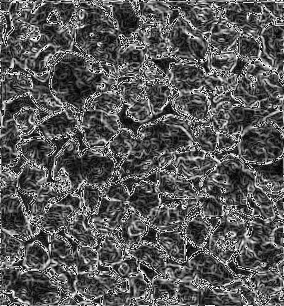
\includegraphics[width=\columnwidth]{edgedetected.png}
    \caption{Imagem resultante da aplicação do Filtro de Sobel à imagem em escala de cinzentos.}
    \label{edgedetection}
\end{figure}
\end{document}
